% TODO make sure quoted values are accurate (i.e. look em up)
\section{Results}
This section is split into two parts, the first looking at the results
of our cloud coverage analysis and the second looking into the NDVI
analysis.
\subsection{Cloud coverage}
Figure \ref{fig:cf_temporal} shows the dynamics of cloud coverage
anomalies between March 2008 and July 2017 for South Africa (Figure
\ref{fig:cf_t_south}) and East Africa (Figure \ref{fig:cf_t_east}) and
associated uncertainty, indicated by the shaded region. Also plotted
are the ONI and the relevant Indian Ocean SST anomalies (SSTAs) -- SWIO
for South Africa and WTIO for East Africa.

\begin{figure*}
  \centering
  \begin{subfigure}{\textwidth}
    \centering
    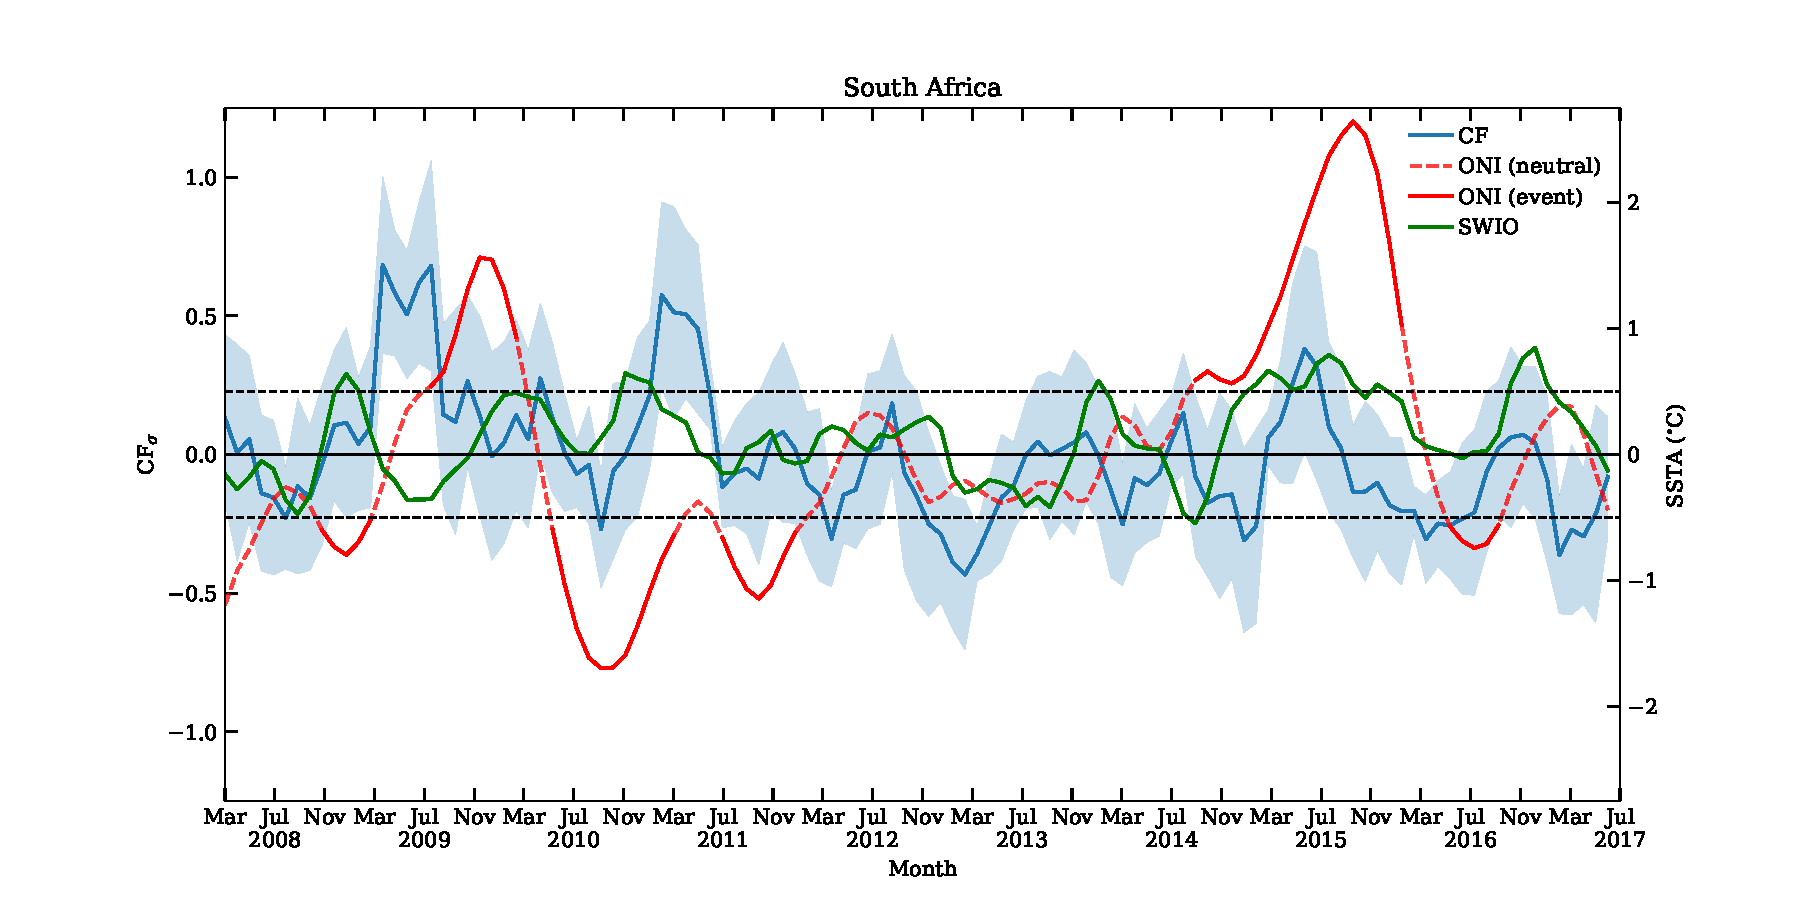
\includegraphics[width=0.85\textwidth]{figures/cf_oni_io_capetown_5window_median}
    \caption{South Africa}
    \label{fig:cf_t_south}
  \end{subfigure}
  \begin{subfigure}{\textwidth}
    \centering
    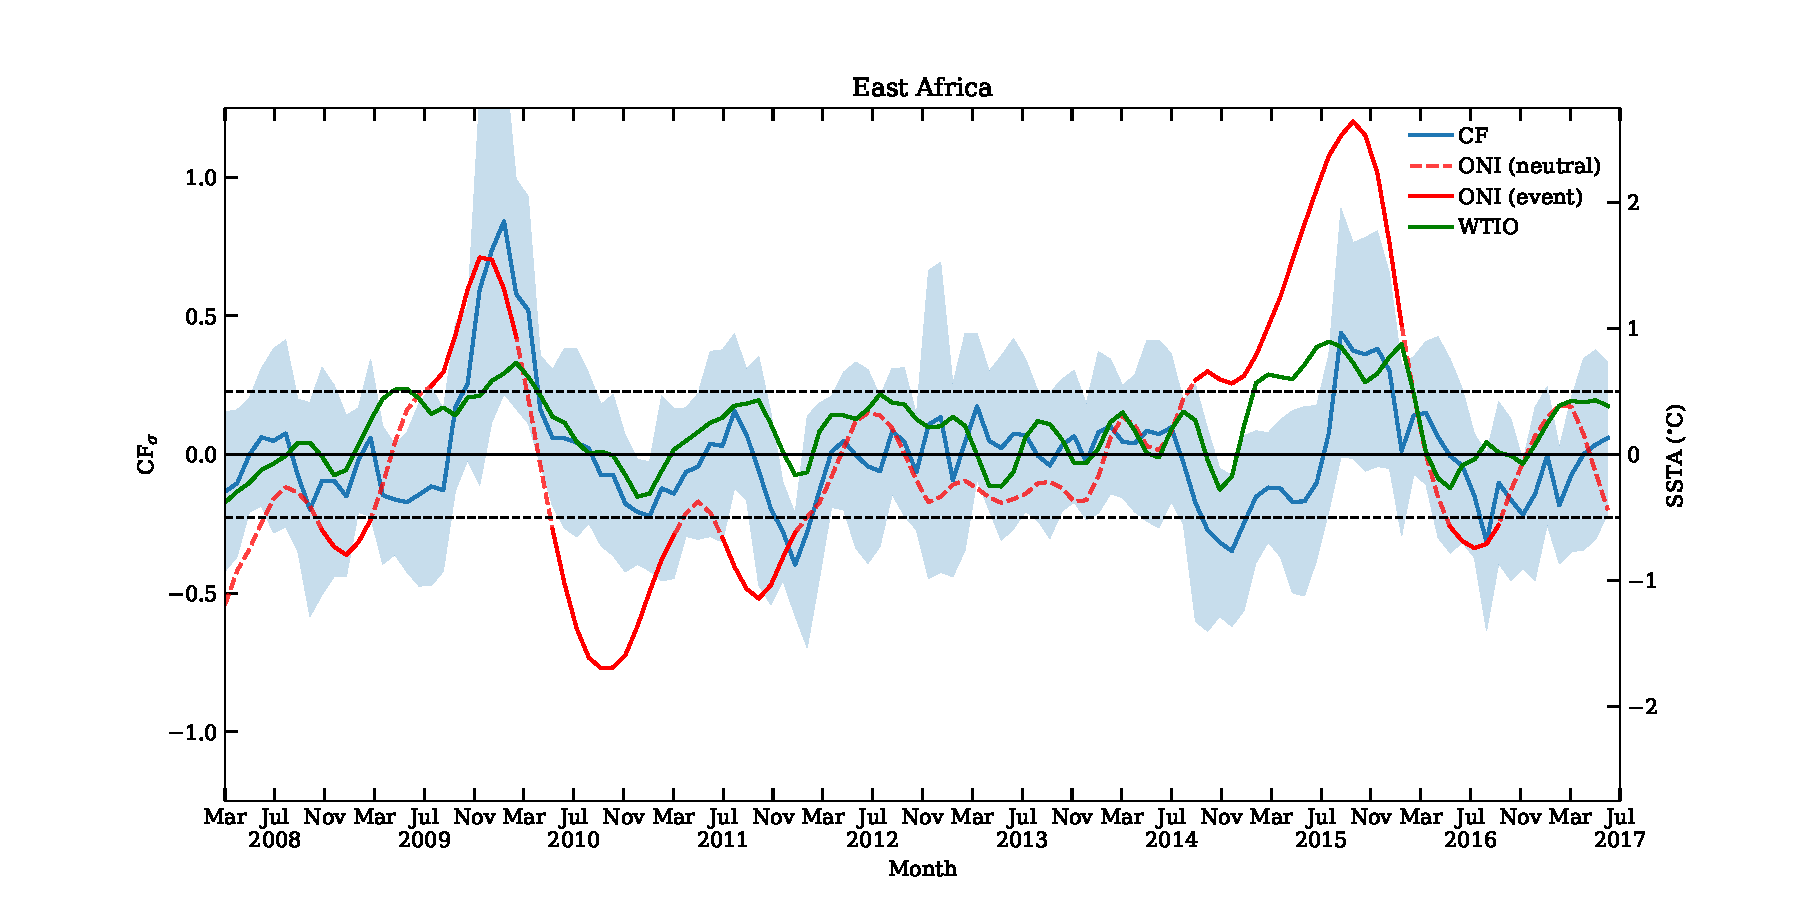
\includegraphics[width=0.85\textwidth]{figures/cf_oni_io_eastafrica_5window_median}
    \caption{East Africa}
    \label{fig:cf_t_east}
    \end{subfigure}
  \caption{Time series of cloud fraction anomalies (blue) and
    uncertainty (shaded blue) from March 2008 to July 2017. Overlaid
    are the ONI (solid red line during ENSO events, dashed red line
    otherwise) and Indian Ocean SST anomalies (SSTA) for the relevant
    part of the Indian Ocean (green, SWIO for South Africa and WTIO
    for East Africa). Dashed black lines indicate the $\pm0.5^{\circ}$C
    threshold for declaring ENSO events. Top panel: South
    Africa. Bottom panel: East Africa. We can see that for South
    Africa, the cloud fraction anomalies are generally anticorrelated
    with ONI during ENSO events with a lag of $\sim2$ months, aside from
    July 2015, where the effect on cloud fraction anomalies appears to
    be dominated by the SWIO SSTAs. For East Africa, cloud fraction
    anomalies appear to be strongly correlated with both ENSO events
    and WTIO SSTAs.}
  \label{fig:cf_temporal}
\end{figure*}

From Figure \ref{fig:cf_t_south} we can see that in many instances, the
cloud fraction anomalies for South Africa appear to be out of phase
with ENSO events, following a lag of $\sim2$ months. For example,
following the peak of the 2010 \nina{} event around November, we
observe a turnaround of cloud fraction anomalies from $-0.25$ to a
peak of $0.5$ by March 2011, which persists until around July of that
year. During the very strong \elnino{} event beginning in November
2014 we observe a positive cloud fraction anomaly, coinciding with
extended periods of positive SWIO SSTAs.

Looking at Figure \ref{fig:cf_t_east} we observe strong positive cloud
fraction anomalies following the peak of the \elnino{} events of
2009/2010 and 2014/2015, again with a lag of $\sim2$ months. However,
cloud fraction anomalies are suppressed during the growth of the
2014/2015 \elnino{} and appear to instead follow the negative WTIO
SSTAs. Negative cloud fraction anomalies are observed during the
2008/2009, 2010/2011, 2011/2012 and 2016 \nina{} events, exhbibiting
the same time lag. During all of these periods, apart from the 2016
\nina{}, negative WTIO SSTAs are also present.



\subsection{NDVI}
\subsubsection{Spatial}
\begin{figure*}
  \centering
  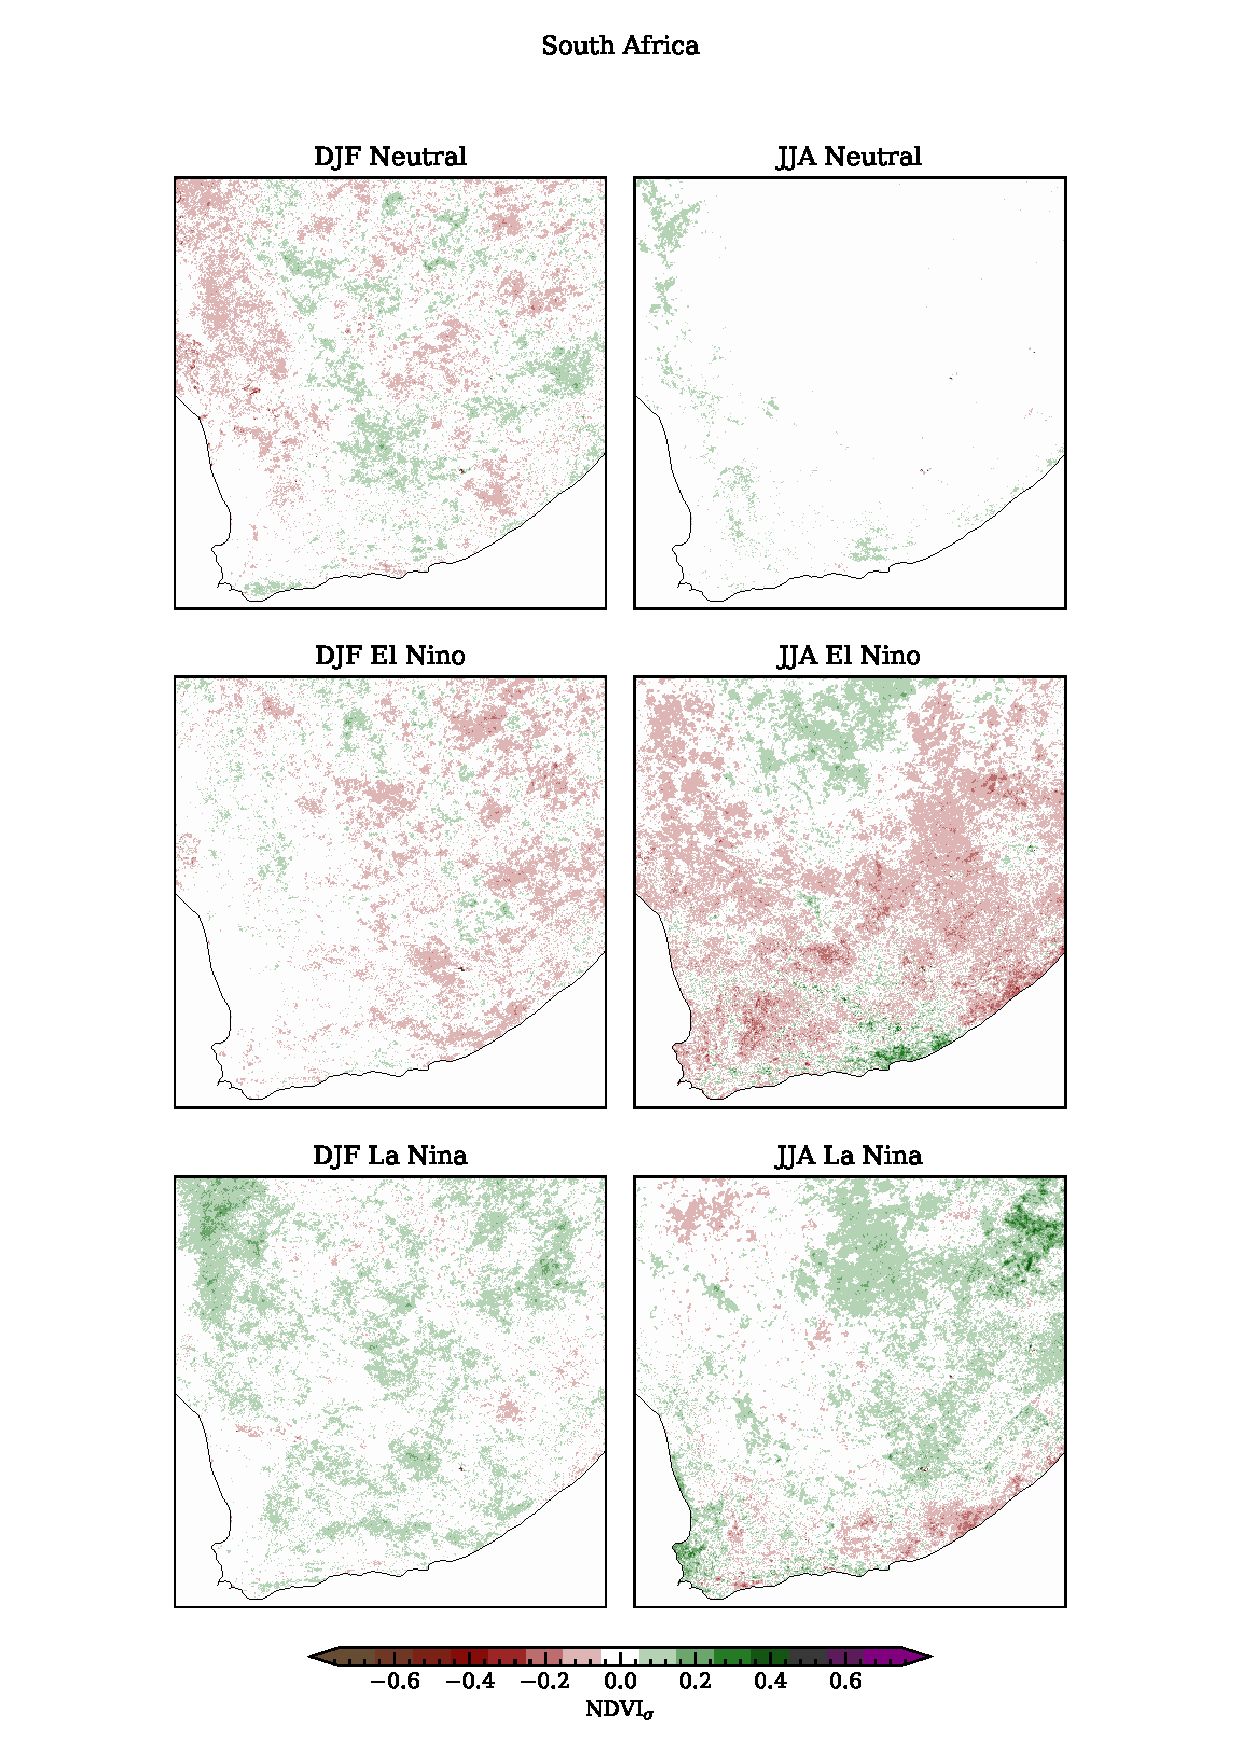
\includegraphics[height=0.9\textheight]{figures/ndvi_spatial_seasonal_anomalies_capetown}
  \caption{Spatial distribution of NDVI anomalies for South
    Africa. Three monthly means are taken for
    December-January-February (DJF) and June-July-August (JJA) and
    averaged again according to which phase of ENSO was present at the
    time.}
  \label{fig:ndvi_sp_south}
\end{figure*}

\begin{figure*}
  \centering
  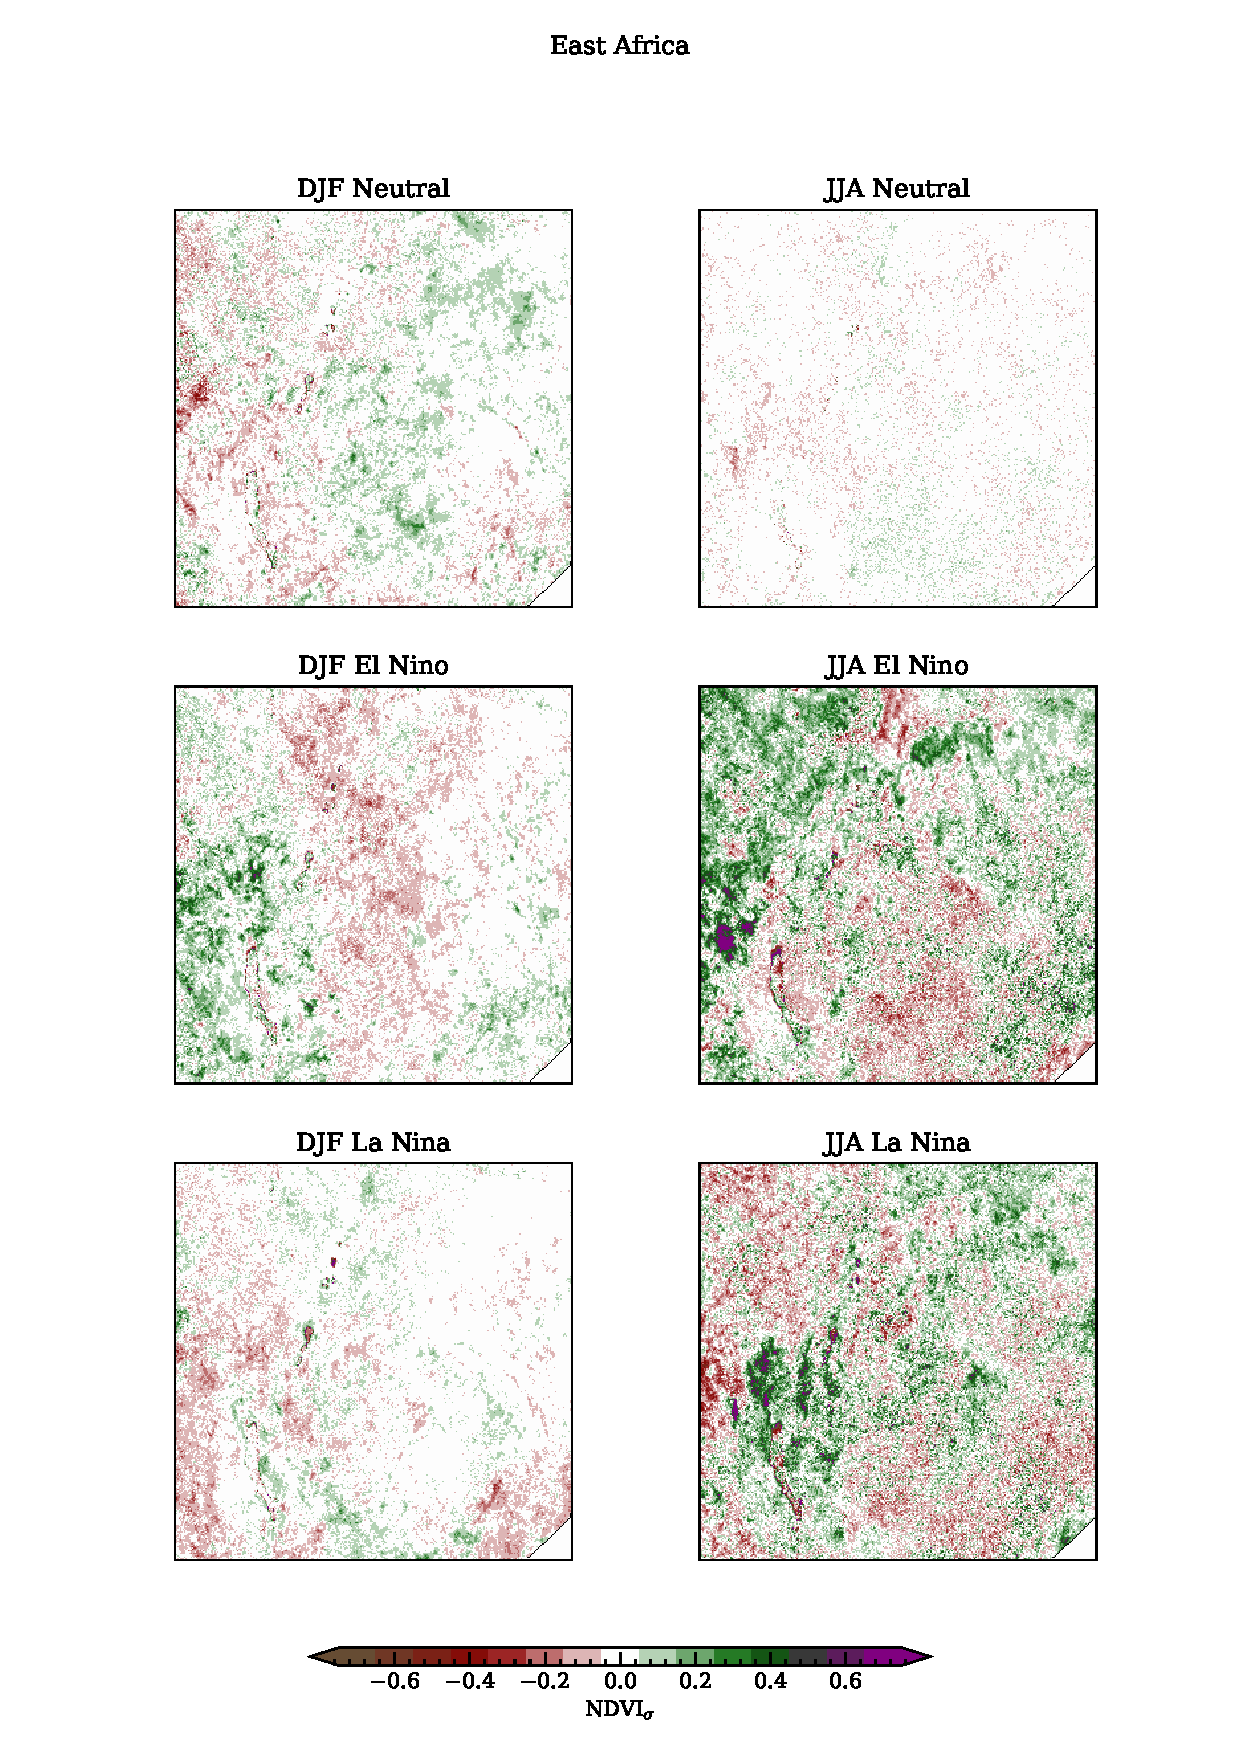
\includegraphics[height=0.9\textheight]{figures/ndvi_spatial_seasonal_anomalies_eastafrica}
  \caption{Spatial distribution of NDVI anomalies for East
    Africa. Three monthly means are taken for
    December-January-February (DJF) and June-July-August (JJA) and
    averaged again according to which phase of ENSO was present at the
    time.}
  \label{fig:ndvi_sp_east}
\end{figure*}

  
